\section{Radio Frequency Interference Analysis}

Based on estimations from the DRAO RFI monitor, we expect to have good visibility for 44 transitions and partial visibility for an additional 27. The number of visible lines per frequency range is presented in table \ref{tbl:RFI_lines}.

\begin{table}[h!]
\centering
\caption{RFI Impact on Transition Line Visibility}
\label{tbl:RFI_lines}

\begin{tabular}{lrr}
\hline
\textbf{Frequency Range (MHz)} & \textbf{Visible Transitions} & \textbf{Partially Visible Transitions} \\
\hline
400--800     & 21 & 19 \\
800--1200    & 11 & 8  \\
1200--1500   & 12 & 0  \\
\hline
\textbf{Total} & \textbf{44} & \textbf{27} \\
\hline
\end{tabular}

\\[4pt]
\textit{Estimates based on DRAO RFI monitor.}

\end{table}

\subsection{Definition of RFI}
Radio frequency interference (RFI) consists of radio waves emitted from any Earthly source that can overcome or be confused with the target signal. Examples of RFI can include satellites, electronic equipment, and local broadband communications. Unlike statistical noise, RFI cannot be removed through smoothing or time averaging because RFI is a distinct signal and not a random variable. Instead, it must be identified and removed.\\

A roof mounted receiver located at the DRAO site called the `RFI monitor' records radio signals from all directions, providing an estimate of the expected RFI which CHORD will receive. There are a few important limitations to consider about conclusions from the RFI monitor:
\begin{itemize}
    \item CHORD is orders of magnitude more sensitive than the RFI monitor, signals that are not detectable by the RFI monitor may nonetheless impede CHORD.
    \item CHORD has a directional beam pointed upwards while the RFI monitor receives signal from all directions. RF signals travelling horizontally or from the surface upwards will be be visible to the RFI monitor but may be absent from CHORD.
    \item RFI changes over time and as new sources emerge, spectrum currently free of RFI might become corrupted.
\end{itemize}

\subsection{Kurtosis based RFI Detection}

Spectral Kurtosis was developed by \citet{nita_statistics_2010} as an unbiased measure of RFI detection. The principle of Kurtosis based methods is that true astronomical signals should appear Gaussian, while RFI should not. Kurtosis is the fourth moment 
where
\begin{align}
    \text{First moment:}  \quad & \E[X] = \frac{1}{n}\sum_{i=1}^{n} x_i
        && \text{(mean, } \mu) \\[4pt]
    \text{Second moment:} \quad & \E[X^2] - \E[X]^2 = \frac{1}{n}\sum_{i=1}^{n} (x_i-\mu)^2
        && \text{(variance, } \sigma^2) \\[4pt]
    \text{Third moment:}  \quad & \frac{\E[(X-\mu)^3]}{\sigma^3}
        = \frac{1}{n}\sum_{i=1}^{n}\!\left(\frac{x_i-\mu}{\sigma}\right)^{3}
        && \text{(skewness)} \\[4pt]
    \text{Fourth moment:} \quad & \frac{\E[(X-\mu)^4]}{\sigma^4}
        = \frac{1}{n}\sum_{i=1}^{n}\!\left(\frac{x_i-\mu}{\sigma}\right)^{4}
        && \text{(kurtosis)}
\end{align}



% \begin{figure}[t]
%     \centering
%     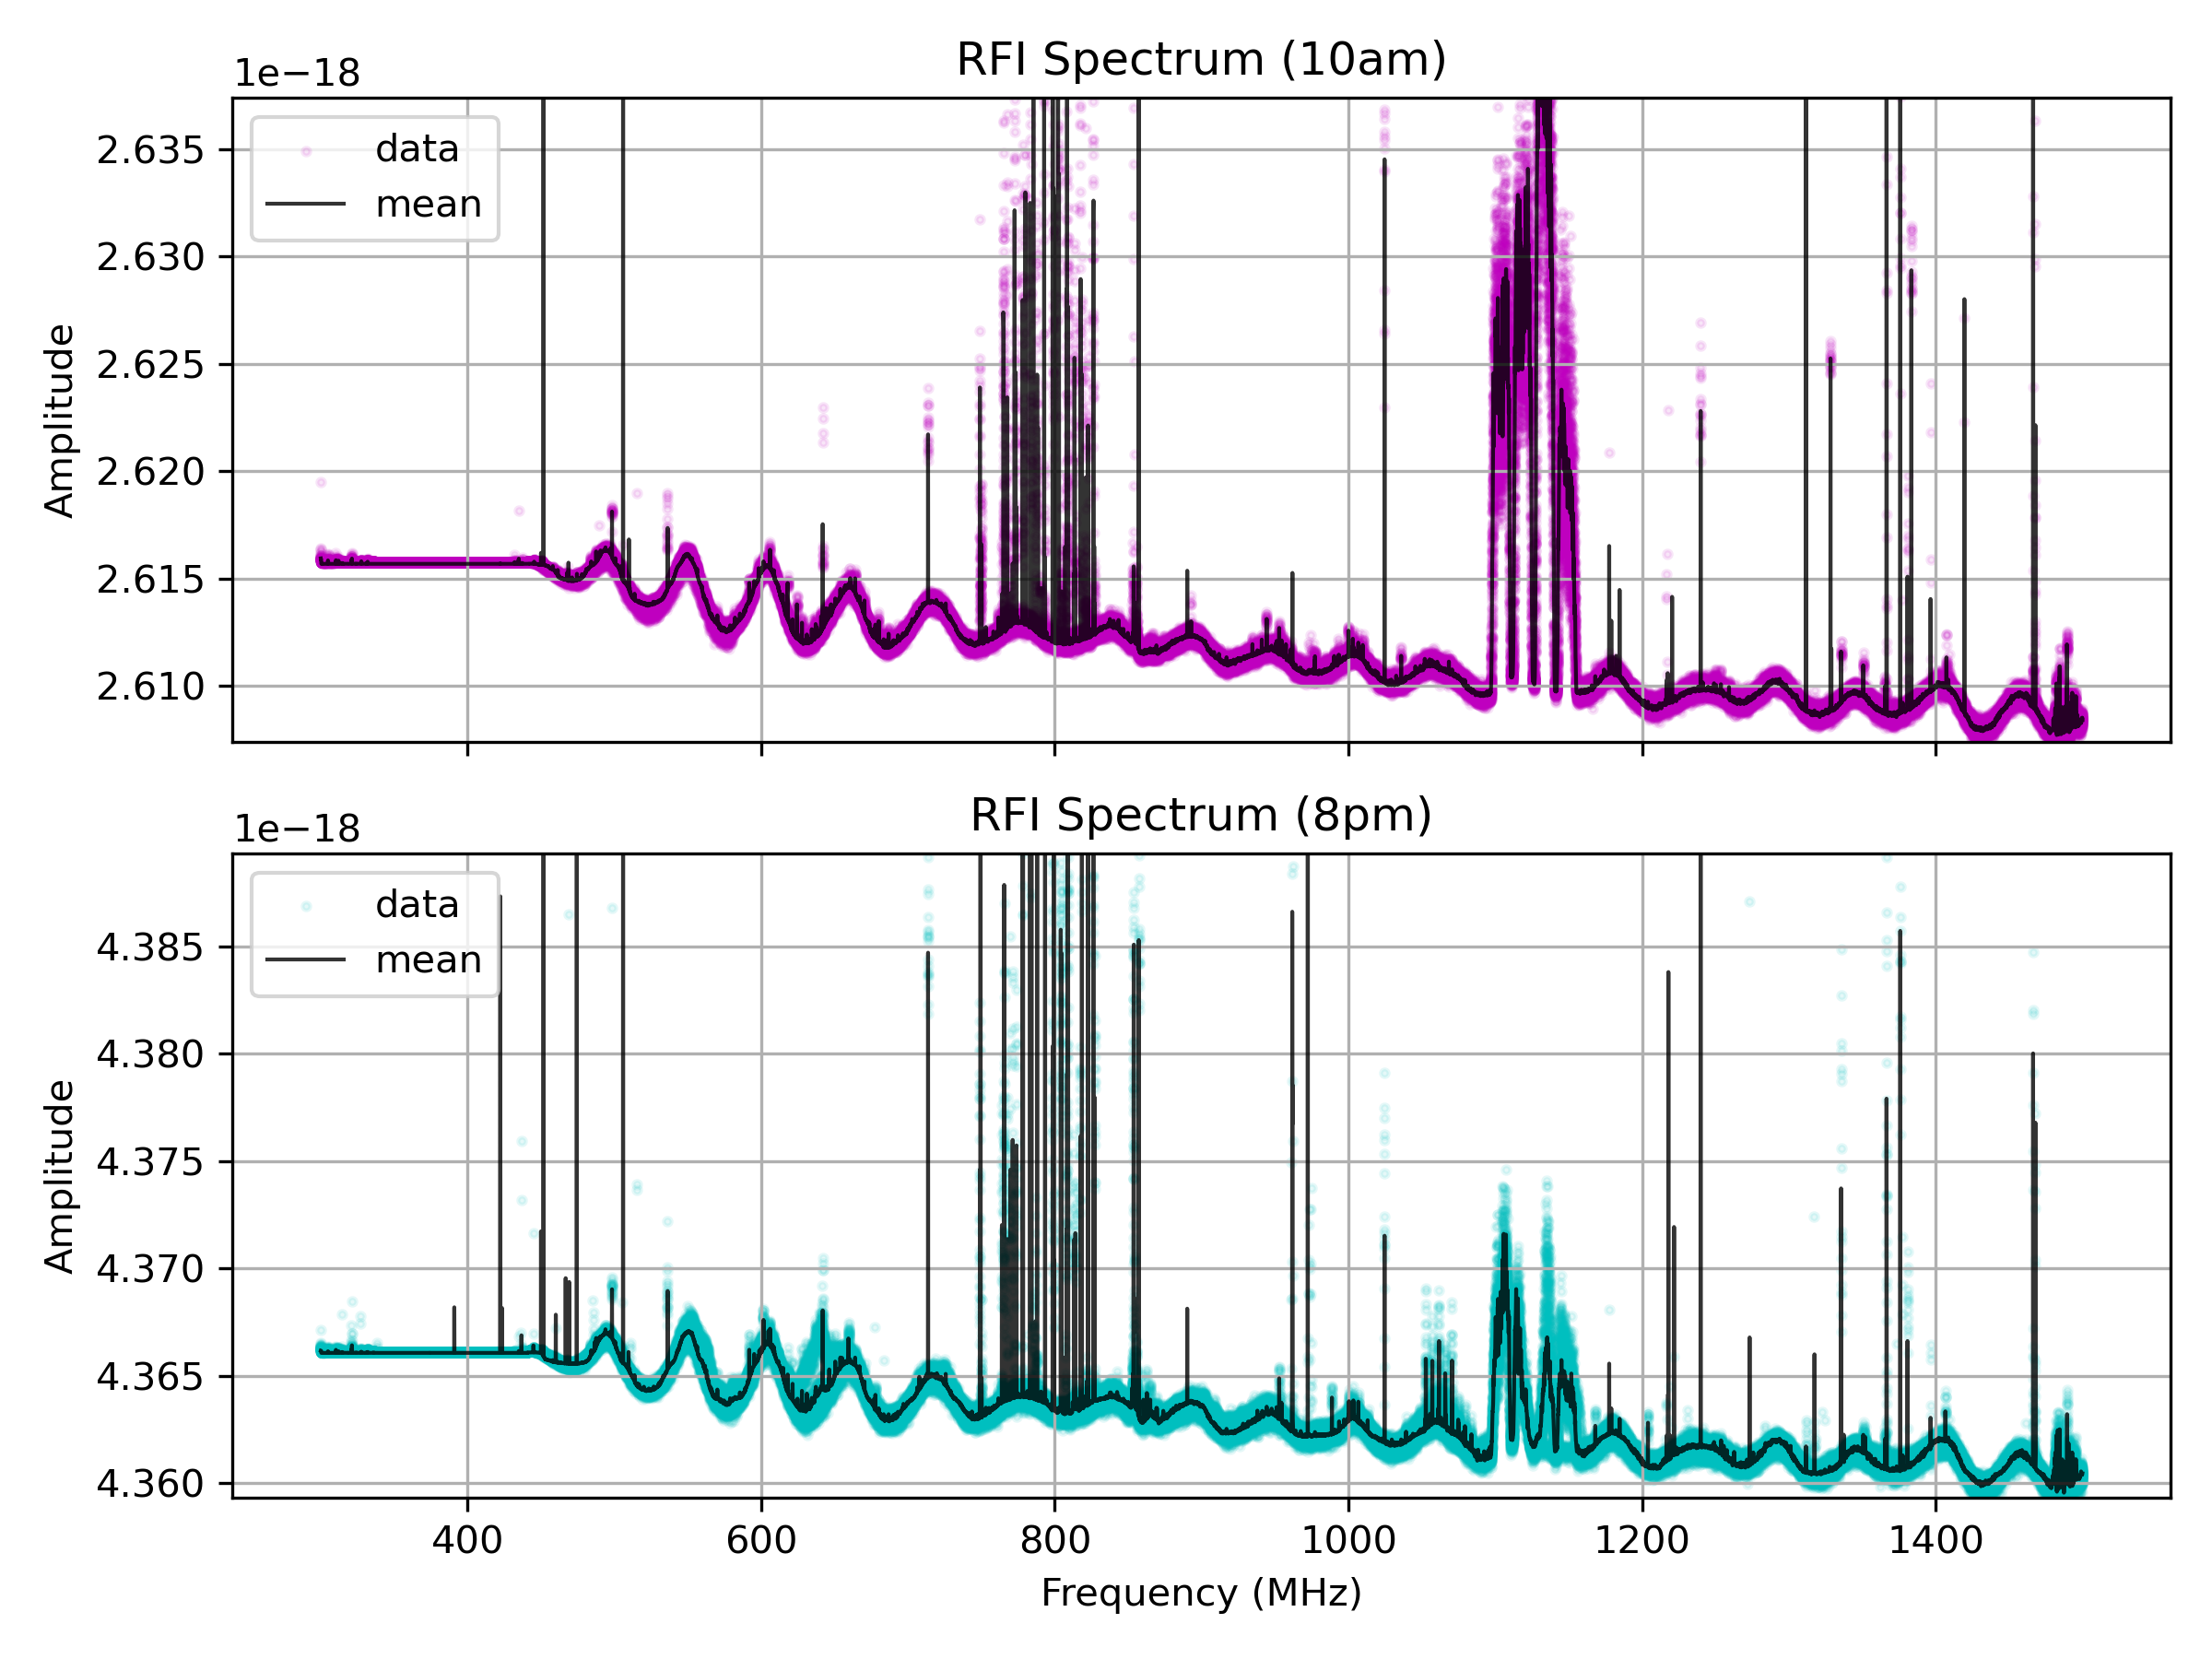
\includegraphics[width=1\linewidth]{thesis/plots/rfi/full_spectrum_overview.png}
%     \caption{Enter Caption}
%     \label{fig:placeholder}
% \end{figure}